\title{CS736: Homework 1}
\author{190050028 Danish Anugral \\190050053 Jayesh Singla\\ 190050114 Shrey Singla}
\date{April 2021}

\documentclass[11pt]{article}

\usepackage{amsmath}
\usepackage{amssymb}
\usepackage{hyperref}
\usepackage{ulem}
\usepackage{parskip}
\usepackage[margin=0.5in]{geometry}
\usepackage{graphicx}
\usepackage{float}
\usepackage{caption}
\usepackage{subcaption}

\setlength{\parskip}{1em}
\begin{document}
\maketitle

\begin{enumerate}
    \item 
    We have implemented the independent and identically distributed Gaussian distribution as the noise model. ie $P(y_i | x_i) \sim \mathbb{G}(0, \sigma^2)$ where $\sigma=1$. We have used simple gradient descent with variable step-size to get the minimum value of the loss function. The step-size ($\eta$) heuristic is as follows: 
    \begin{enumerate}
        \item if the loss function decreases, $\eta = \eta*1.1$
        \item if the loss function increases, $\eta = \eta*0.5$
    \end{enumerate}
    The breaking condition is that the loss function value between consecutive iterations is less than 0.001 (maximum iterations 1000). We allow it to run for atleast 100 iterations for warmup. \\
    
    The fine-tuning is done in coarse-to-fine manner using grid-search approach. First both $\alpha$ and $\gamma$ are searched between 0 to 1 using 0.1 step-size. Once their optimal values are obtained, the range of search is decreased till acceptable accuracy is obtained.
    \begin{enumerate}
        \item RRMSE between noisy and noiseless images is 0.2986
        \item 
        \begin{tabular}{|c|c|c|c|}
            \hline
             Prior & Quadratic & Huber & Discontinuity adaptive  \\
             \hline
             $\alpha*$ & 0.1015 &0.99333 &0.99\\
             \hline
             $\gamma*$ & - &0.00072 &0.001\\
             \hline
            RRMSE*($\alpha*$,$\gamma*$)& 0.281269 &0.235916 & 0.236343\\
            \hline
             RRMSE*($0.8\alpha*$,$\gamma*$)& 0.281723 &0.291113& 0.288724\\
            \hline
             RRMSE*($1.2\alpha*$,$\gamma*$)& 0.281656 &0.237318 & 0.238166\\
            \hline
            RRMSE*($\alpha$*,1.2$\gamma$*)& - &0.236245 & 0.236404\\
            \hline
             RRMSE*($\alpha$*,0.8$\gamma$*)& - &0.237308 & 0.236566\\
             \hline
        \end{tabular}
        \item 
        \begin{figure}[H]
            \centering
            \begin{subfigure}[b]{0.4\textwidth}
                 \centering
                 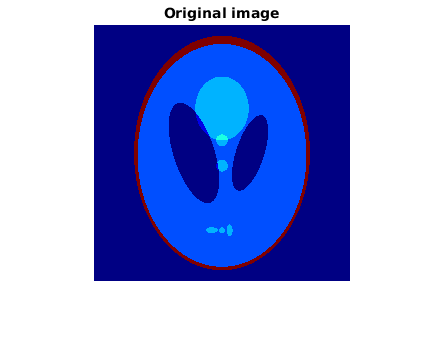
\includegraphics[width=\textwidth]{Plots/Ques1/1-original.png}
                 \caption{Noiseless image}
            \end{subfigure}
            \begin{subfigure}[b]{0.4\textwidth}
                 \centering
                 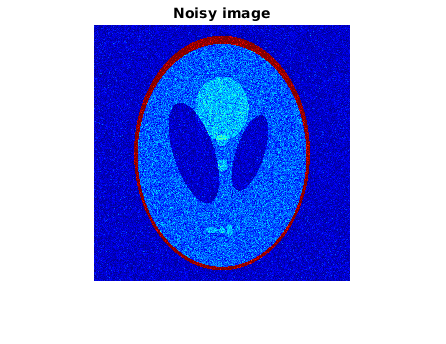
\includegraphics[width=\textwidth]{Plots/Ques1/1-noisy.png}
                 \caption{Noisy Image}
            \end{subfigure}
            \begin{subfigure}[b]{0.4\textwidth}
                 \centering
                 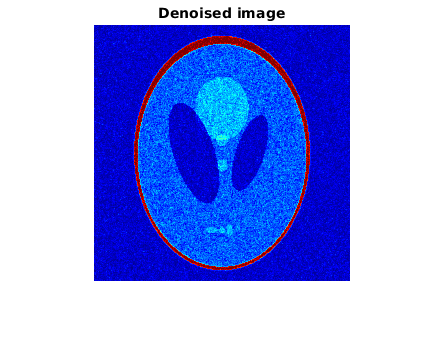
\includegraphics[width=\textwidth]{Plots/Ques1/1-quadratic_denoised.png}
                 \caption{Denoising with Quadratic function g1() with optimal parameters}
            \end{subfigure}
            \begin{subfigure}[b]{0.4\textwidth}
                 \centering
                 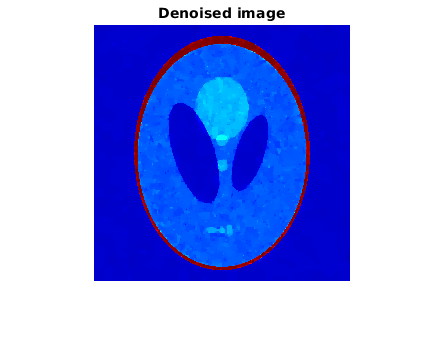
\includegraphics[width=\textwidth]{Plots/Ques1/1-huber_denoised.png}
                 \caption{Denoising with Huber function g2() with optimal parameters}
            \end{subfigure}
            \begin{subfigure}[b]{0.4\textwidth}
                 \centering
                 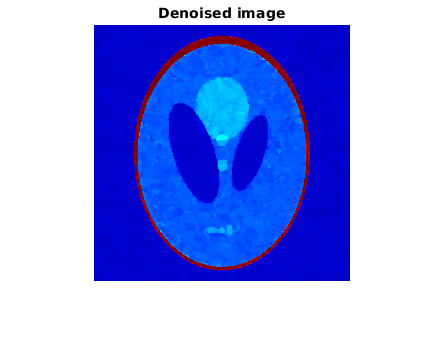
\includegraphics[width=\textwidth]{Plots/Ques1/1-denoised_discontinuity.png}
                 \caption{Denoising with Discontinuity adaptive function g3() with optimal parameters}
            \end{subfigure}
            \caption{Results of denoising}
            \label{fig:my_label}
        \end{figure}
        
        \item \begin{figure}[H]
            \centering
            \begin{subfigure}[b]{0.4\textwidth}
                 \centering
                 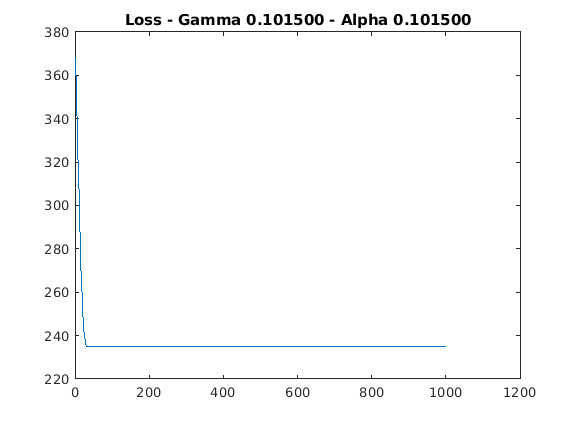
\includegraphics[width=\textwidth]{Plots/Ques1/1-quadratic_loss.png}
                 \caption{Quadratic Function g1()}
            \end{subfigure}
            \begin{subfigure}[b]{0.4\textwidth}
                 \centering
                 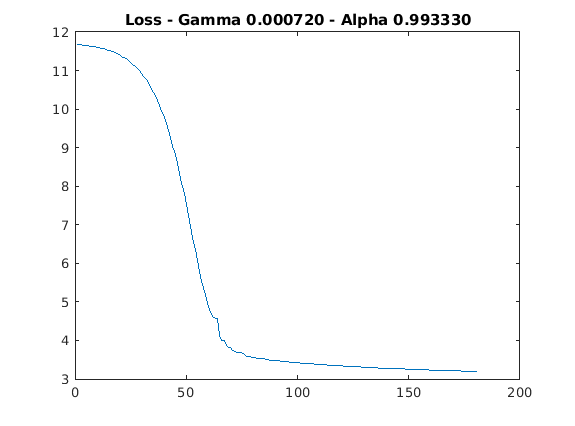
\includegraphics[width=\textwidth]{Plots/Ques1/1-huber_loss.png}
                 \caption{Huber Function g2()}
            \end{subfigure}
            \begin{subfigure}[b]{0.4\textwidth}
                 \centering
                 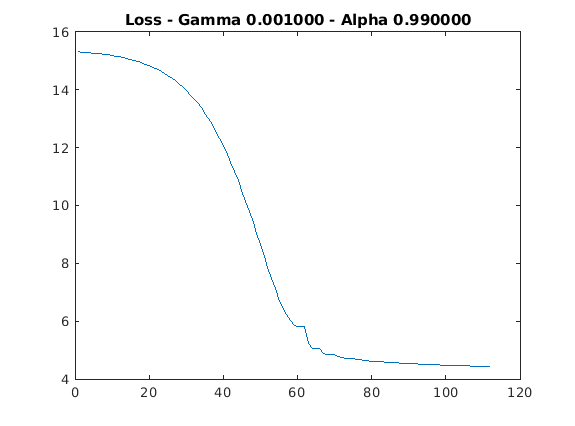
\includegraphics[width=\textwidth]{Plots/Ques1/1-discontinuity_loss.png}
                 \caption{Discontinuity adaptive function g3()}
            \end{subfigure}
            
            \caption{Loss function (negative log posterior) versus iterations}
            \label{fig:my_label}
        \end{figure}
        \item Instructions to run code: Navigate the the 'code' directory and run the code 'main.m'. The code is well commented. The main denoising algorithm is present in 'denoise.m' and 'main.m' performs the hyperparameter tuning for $\alpha$ and $\gamma$ for both images and all three priors.  
    \end{enumerate}
    
%%%%%%%%%%%%%%%%%%%%%%%%%%%%%%%%%%%%%%%%%%%%%%%%%%%%%%%%%%%%%%%%%%%%%%%%%%%%%%%%%%
    \item 
    We have implemented the independent and identically distributed Gaussian distribution as the noise model. ie $P(y_i | x_i) \sim \mathbb{G}(0, \sigma^2)$ where $\sigma=1$
    \begin{enumerate}
        \item RRMSE between noisy and noiseless images is 0.1424
        \item 
         \begin{tabular}{|c|c|c|c|}
            \hline
             Prior & Quadratic & Huber & Discontinuity adaptive  \\
             \hline
             $\alpha*$ & 0.1344 &0.53 &0.643\\
             \hline
             $\gamma*$ & - & 0.0038 &0.033888\\
             \hline
            RRMSE*($\alpha*$,$\gamma*$).  & 0.122171 & 0.113725 & 0.114508\\
            \hline
             RRMSE*($0.8\alpha*$,$\gamma*$) & 0.122702 & 0.116441 & 0.117746\\
            \hline
             RRMSE*($1.2\alpha*$,$\gamma*$) & 0.122615 & 0.116460 & 0.121356\\
            \hline
            RRMSE*($\alpha$*,1.2$\gamma$*) & - & 0.114192 & 0.115031\\
            \hline
             RRMSE*($\alpha$*,0.8$\gamma$*) & - & 0.114316  & 0.114636\\
             \hline
        \end{tabular}
        
        
        % \begin{tabular}{|p{2cm}|p{2cm}|p{2cm}|p{2cm}|p{2cm}|p{2cm}|p{2cm}|}
        %     \hline
            
        %     Prior & $\alpha^*$ & $\gamma^*$ &
        %     RRMSE($\alpha^*$,$\gamma^*$) &
        %     RRMSE($1.2\alpha^*$,$\gamma^*$) & RRMSE($0.8\alpha^*$,$\gamma^*$) & RRMSE($\alpha^*$,$1.2\gamma^*$) & RRMSE($\alpha^*$,$0.8\gamma^*$)  \\
        %     \hline
        %     \hline
        %     Quadratic & - & - & - & - & - & - \\
        %     \hline
        %     Huber & 0.99333 & 0.000842 & 0.235 &  & - & - \\
        %     \hline
        %     Discontinuity adaptive & - & - & - & - & - & - \\
        %     \hline
        % \end{tabular}
        \item 
        \begin{figure}[H]
            \centering
            \begin{subfigure}[b]{0.4\textwidth}
                 \centering
                 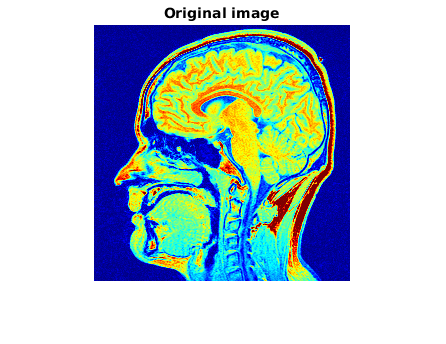
\includegraphics[width=\textwidth]{Plots/Ques2/2-original.png}
                 \caption{Noiseless image}
            \end{subfigure}
            \begin{subfigure}[b]{0.4\textwidth}
                 \centering
                 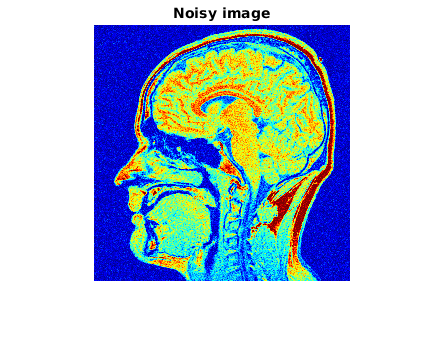
\includegraphics[width=\textwidth]{Plots/Ques2/2-noisy.png}
                 \caption{Noisy Image}
            \end{subfigure}
            \begin{subfigure}[b]{0.4\textwidth}
                 \centering
                 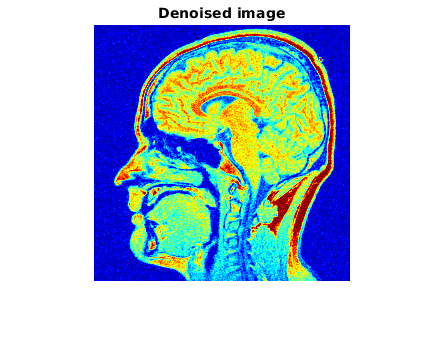
\includegraphics[width=\textwidth]{Plots/Ques2/2-quadratic_denoised.png}
                 \caption{Denoising with Quadratic function g1() with optimal parameters}
            \end{subfigure}
            \begin{subfigure}[b]{0.4\textwidth}
                 \centering
                 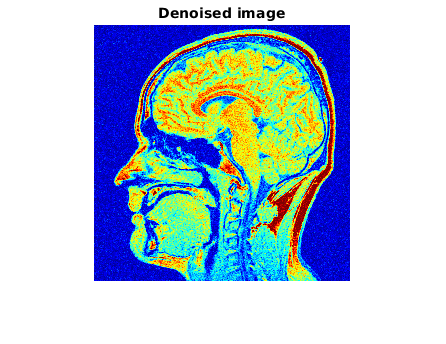
\includegraphics[width=\textwidth]{Plots/Ques2/2-huber_denoised.png}
                 \caption{Denoising with Huber function g2() with optimal parameters}
            \end{subfigure}
            \begin{subfigure}[b]{0.4\textwidth}
                 \centering
                 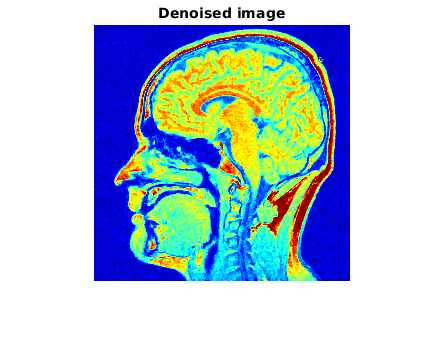
\includegraphics[width=\textwidth]{Plots/Ques2/2-discontinuity_denoised.png}
                 \caption{Denoising with Discontinuity adaptive function g3() with optimal parameters}
            \end{subfigure}
            \caption{Results of denoising}
            \label{fig:my_label}
        \end{figure}
        
        \item \begin{figure}[H]
            \centering
            \begin{subfigure}[b]{0.4\textwidth}
                 \centering
                 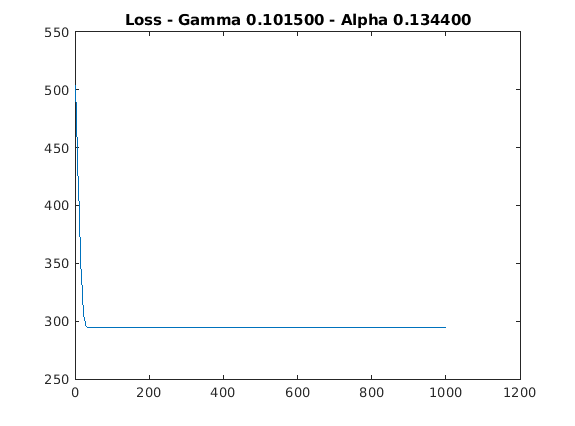
\includegraphics[width=\textwidth]{Plots/Ques2/2-quadratic_loss.png}
                 \caption{Quadratic Function g1()}
            \end{subfigure}
            \begin{subfigure}[b]{0.4\textwidth}
                 \centering
                 \includegraphics[width=\textwidth]{Plots/Ques2/2-huber_loss.png}
                 \caption{Huber Function g2()}
            \end{subfigure}
            \begin{subfigure}[b]{0.4\textwidth}
                 \centering
                 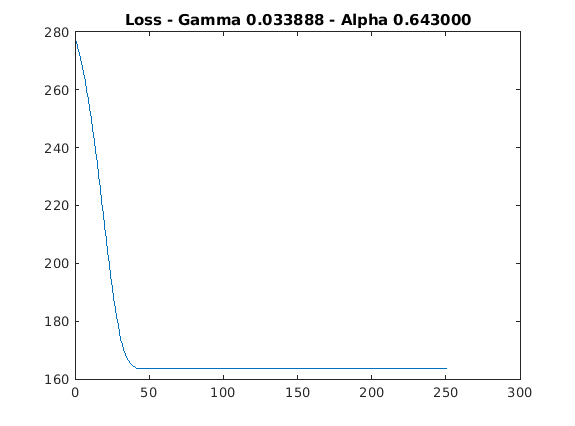
\includegraphics[width=\textwidth]{Plots/Ques2/2-discontinuity_loss.png}
                 \caption{Discontinuity adaptive function g3()}
            \end{subfigure}
            
            \caption{Loss function (negative log posterior) versus iterations}
            \label{fig:my_label}
        \end{figure}
    \end{enumerate}
    
%%%%%%%%%%%%%%%%%%%%%%%%%%%%%%%%%%%%%%%%%%%%%%%%%%%%%%%%%%%%%%%%%%%%%%%%%%%%%%%%%%
    \item \begin{enumerate}
        \item We first observe that the major difference between an RGB image and a grayscale image is that there are three values at each pixel and thus we need to capture correlation across channels as well. Another thing to note is that it is difficult to directly model the dependency of pixel values across channels, thus we would be model each 3-valued pixel vector as a 3-dimensional random variable with 4 neighbours as the pixel vectors at adjacent positions. 
        
        Thus, a clique contains 6 elements, with 3 elements each from adjacent pixel vectors. We want to model the vector such that the change in any dimension across neighbours is small except at discontinuity/outliers.
        
        Also, we observe that a better way to characterize smoothness in images would be to consider the HSV representation of a pixel instead of the RGB one as a large change in RGB norm may not always correspond to a discontinuity/outlier. The semantic independence between the 3 values in HSV better ensures that a a large change corresponds to a more prominent discontinuity/outlier. In other words, for RGB image, a change in pixel R implies a large change in pixels G and B (due to dependency between color channels), which is difficult to model. Such dependency does not exist in HSV color space.
        
        Thus, the potential function for a clique c (2 adjacent pixels) can be modeled as - 
        
        $$
        V_c(\boldsymbol{x_{ij}},\boldsymbol{x_{i'j'}}) = g(||h(\boldsymbol{x_{ij}}) - h(\boldsymbol{x_{i'j'}})||_2)
        $$
        
        where g is the Huber function and h is the HSV tranform
        
        Thus, the prior model for the image is 
        
        $$
        P(X) = \frac{1}{Z}e^{-\frac{1}{T}\sum_{c \in C} V_c(\{\boldsymbol{x}_c\})}
        $$
        
        \item A suitable noise model for microscopy RGB images would be channel-independent Gaussian noise.
        
        Let $x_{ij}^k,y_{ij}^k$ be the pixel values at position (i,j) and channel k.
        
        The noise model is as follows - 
        
        $$
        y_{ij}^k = x_{ij}^k + N(0,\sigma^2)
        $$
        $$
        P(y_{ij}^k | x_{ij}^k) = \frac{1}{\sqrt{2\pi\sigma^2}}e^{-\frac{(y_{ij}^k - x_{ij}^k)^2}{2\sigma^2}}
        $$
        
        $$
        P(Y|X) = \prod_{i,j,k} P(y_{ij}^k | x_{ij}^k)
        $$
        
        Another possible solution to formulating the noise model would be to model the noise in the pixel vector as a zero multi-variate Gaussian where the noise in individual channels is not necessarily independent. 
        The covariance matrix would have to be inferred using a data-driven approach.
        
        \item The Bayesian denoising formulation would be maximising the posterior. Let the observed image be $y$, where each pixel has 3 values associated to it. Let the random variable associated with denoised image be X. Let the parameters of the model be $\theta$.
        We need to maximise $P(X | y, \theta)$
        \begin{align*}
            P(X | y, \theta) &= P(X_i, X_{\sim i} | y, \theta)\\
            &= P(X_i | X_{\sim i}, y, \theta) P(X_{\sim i} | y, \theta)\\
            &= P(X_i | X_{N_i}, y_i, \theta) P(X_{\sim i} | y, \theta)\\
        \end{align*}

        \begin{align*}
            \implies \max_{x_i} P(X | y, \theta) &= \max_{x_i} P(X_i | X_{N_i}, y_i, \theta) P(X_{\sim i} | y, \theta)\\
            &= \max_{x_i} P(X_i | X_{N_i}, y_i, \theta)\\
            &= \max_{x_i} \frac{P (y_i | X_i, X_{N_i}, \theta) P(X_i | X_{N_i}, \theta)}{P (y_i | X_{N_i},\theta)}\\
            &= \max_{x_i} P (y_i | X_i, X_{N_i}, \theta) \\
            &= \max_{x_i} P(y_i | X_i, \theta) P(X_i | X_{N_i}, \theta)
        \end{align*}
        \begin{equation*}
            \implies argmax_{x_i} P(X|y_i, \theta) = argmax_{x_i} \left[\log P(y_i|X_i, \theta) + \log P(X_i | X_{N_i}, \theta)\right]
        \end{equation*}
        $$
            P(y_i | X_i, \theta) = \prod_{i,j,k} P(y_{i,j}^k | x_{i,j}^k) 
        $$
        $$
           \implies \log P(y_i | X_i, \theta) \propto \sum_{i,j,k} -\frac{(y_{ij}^k - x_{i,j}^k)^2}{\sigma^2}
        $$
        Where $\sigma$ is the std dev of the noise distribution.
        Also, 
        $$
        \log P(X_i | X_{N_i}, \theta) \propto \sum_{c \in C}- V_c(\{x_c\})
        $$
        Hence, the Bayesian denoising formulation results in the image by solving the optimisation problem as follows:
        
        $$
        \min \left[\sum_{i,j,k} \frac{(y_{i,j}^k - x_{i,j}^k)^2}{\sigma^2} + \sum_{c \in C} V_c(\{x_c\})\right]
        $$
        
        
    \end{enumerate}
\end{enumerate}


\end{document}
